\documentclass{beamer}

\usepackage{hyperref}
\usepackage{tikz}

\title{Red Queen's Sync Protocol for Ethereum}
\author{Andrew Ashikhmin \& Alexey Akhunov}
\date{Ethereum Core Dev Meeting\\ April 2019, Berlin}

\begin{document}
  \frame{\titlepage}

  \begin{frame}
    \frametitle{Motivation}
    \begin{itemize}
      \item Current eth/63 snapshot sync (fast sync) is slow (a few hours for full nodes).
      \item Growing state size can potentially lead to sync failures due to history pruning.
      \item Parity's warp sync is vulnerable to a "rubbish data" attack.
      \item A number of similar proposals are emerging: Leaf Sync, Firehose.
      \item We also propose a sync algorithm with an in-depth performance and convergence analysis.
      \item The new protocol caters for light clients (e.g. Mustekala).
      \item Grand vision: swarms of light Ethereum nodes running on mobile, not unlike BitTorrent and Pied Piper :)
      \end{itemize}
  \end{frame}

  \begin{frame}
    \frametitle{Protocol 1/6}

    \textbf{GetBytecode} (0x20)

    [reqID: $\mathbb{N}$,
    [codeHash$_0$: $\mathbb{B}_{32}$, codeHash$_1$: $\mathbb{B}_{32}$, ...]]
    \medskip
    
    Request EVM code of smart contracts.
    The operative is just like $\texttt{GetNodeData}$, except:
    \begin{enumerate}
    \item includes a request ID;
    \item will only return bytecode with the corresponding hash, not arbitrary node data.
    \end{enumerate}
    \bigskip
    
    \textbf{Bytecode} (0x21)
    
    [reqID: $\mathbb{N}$,
    [code$_0$: $\mathbb{B}$, code$_1$: $\mathbb{B}$, ...]]
    \medskip
    
    Reply to $\texttt{GetBytecode}$.
    Bytecode position in the response list must correspond to the position in the request list;
    an empty list should be used for omitted bytecodes.

  \end{frame}

  \begin{frame}
    \frametitle{Protocol 2/6}

    \textbf{GetStateNodes} (0x22)

    [reqID: $\mathbb{N}$, blockHash: $\mathbb{B}_{32}$,
    [prefix$_0$: $\mathbb{Y}$, prefix$_1$: $\mathbb{Y}$, ...]]
    \medskip
    
    Request state trie nodes as of a specific block.
    Note that this operative is similar to $\texttt{GetNodeData}$,
    but it uses prefixes rather than hashes as node keys.
    It will also only return nodes from the state trie,
    not arbitrary node data.

    \bigskip
    
    \textbf{StateNodes} (0x23)
    
    [reqID: $\mathbb{N}$,
    [node$_0$: $\mathbb{B}$, node$_1$: $\mathbb{B}$, ...],
    [availableBlock$_0$: $\mathbb{B}_{32}$, ...]$_{opt}$]
    \medskip
    
    Reply to $\texttt{GetStateNodes}$.
    An empty list returned instead of a node means that the peer does not have enough information about the node requested.
    In that case the peer should return blocks for which requested nodes are available
    (as a list of $\texttt{availableBlock}$ hashes).

  \end{frame}

  \begin{frame}
    \frametitle{Protocol 3/6}

    \textbf{GetAccounts} (0x24)

    [reqID: $\mathbb{N}$, blockHash: $\mathbb{B}_{32}$, [prefix$_0$: $\mathbb{Y}$, prefix$_1$: $\mathbb{Y}$, ...]]
    
    \bigskip

    \textbf{Accounts} (0x25)

[reqID: $\mathbb{N}$,

\quad [

\qquad [status$_0$: $\mathbb{N}$, [[key$^0_{0}$: $\mathbb{B}_{32}$, val$^0_{0}$: $\mathbb{B}$], [key$^1_{0}$: $\mathbb{B}_{32}$, val$^1_{0}$: $\mathbb{B}$], ...]$_{opt}$],

\qquad [status$_1$: $\mathbb{N}$, [[key$^0_{1}$: $\mathbb{B}_{32}$, val$^0_{1}$: $\mathbb{B}$], [key$^1_{1}$: $\mathbb{B}_{32}$, val$^1_{1}$: $\mathbb{B}$], ...]$_{opt}$],

\qquad ...

\quad ],

\quad [availableBlock$_0$: $\mathbb{B}_{32}$, ...]$_{opt}$

]
\medskip

The peer may only return either all leaves of a subtrie or nothing.
$\texttt{status}$ must take one of the following values:
\begin{itemize}
\item 0 -- success;
\item 1 -- no data as of the requested block;
\item 2 -- too many leaves matching the prefix.
\end{itemize}

\end{frame}

\begin{frame}
  \frametitle{Protocol 4/6}

  \textbf{GetStorageSizes} (0x26)

  [reqID: $\mathbb{N}$, blockHash: $\mathbb{B}_{32}$,
  [addressHash$_0$: $\mathbb{B}_{32}$, addressHash$_1$: $\mathbb{B}_{32}$, ...]]
  \medskip
  
  Request storage trie sizes as of a specific block.

  \bigskip
  
  \textbf{StorageSizes} (0x27)
  
  [reqID: $\mathbb{N}$,
  [numLeaves$_0$: $\mathbb{N} | \varnothing$, numLeaves$_1$: $\mathbb{N} | \varnothing$, ...],
  [availableBlock$_0$: $\mathbb{B}_{32}$, ...]$_{opt}$]
  \medskip
  
  Reply to $\texttt{GetStorageSizes}$.
  The peer may return an empty list $\varnothing$ instead of the number of leaves for accounts it does not have enough information about.
  In that case the peer should return blocks for which requested data is available.  

\end{frame}

\begin{frame}
  \frametitle{Protocol 5/6}

  \textbf{GetStorageNodes} (0x28)

  [reqID: $\mathbb{N}$, blockHash: $\mathbb{B}_{32}$,
  
  \quad [addressHash$^0$: $\mathbb{B}_{32}$, [prefix$^0_0$: $\mathbb{Y}$, prefix$^0_1$: $\mathbb{Y}$, ...]],
  
  \quad [addressHash$^1$: $\mathbb{B}_{32}$, [prefix$^1_0$: $\mathbb{Y}$, prefix$^1_1$: $\mathbb{Y}$, ...]],
  
  \quad ...
  
  ]
  \bigskip

  \textbf{StorageNodes} (0x29)

[reqID: $\mathbb{N}$,

\quad [

\qquad [node$^0_0$: $\mathbb{B}$, node$^0_1$: $\mathbb{B}$, ...],

\qquad [node$^1_0$: $\mathbb{B}$, node$^1_1$: $\mathbb{B}$, ...],

\qquad ...

\quad ],

\quad [availableBlock$_0$: $\mathbb{B}_{32}$, ...]$_{opt}$

]

\end{frame}

\begin{frame}
  \frametitle{Protocol 6/6}

  \textbf{GetStorageData} (0x2a)

  [reqID: $\mathbb{N}$, blockHash: $\mathbb{B}_{32}$,
  
  \quad [addressHash$^0$: $\mathbb{B}_{32}$, [prefix$^0_0$: $\mathbb{Y}$, prefix$^0_1$: $\mathbb{Y}$, ...]],
  
  \quad [addressHash$^1$: $\mathbb{B}_{32}$, [prefix$^1_0$: $\mathbb{Y}$, prefix$^1_1$: $\mathbb{Y}$, ...]],
  
  \quad ...
  
  ]
  \bigskip

  \textbf{StorageData} (0x2b)
  \nopagebreak
  
  [reqID: $\mathbb{N}$,
  
  \quad [
  
  \qquad [
  
  \quad \qquad [status$^0_0$: $\mathbb{N}$, [[key$^0_{00}$: $\mathbb{B}_{32}$, val$^0_{00}$: $\mathbb{B}$], ...]$_{opt}$],
  
  \quad \qquad [status$^0_1$: $\mathbb{N}$, [[key$^0_{10}$: $\mathbb{B}_{32}$, val$^0_{10}$: $\mathbb{B}$], ...]$_{opt}$],
  
  \quad \qquad ...
  
  \qquad ],
  
  \qquad ...
  
  \quad ], [availableBlock$_0$: $\mathbb{B}_{32}$, ...]$_{opt}$
  
  ]

\end{frame}

\begin{frame}
  \frametitle{Suggested Sync Algorithm 1/2}

  \begin{itemize}
    \item Always request data as of the most recent block.
    \item Phase 1: get all leaves, probably as of different blocks.
    \item Simultaneously request necessary intermediate nodes to verify the leaves.
    \item Keep the top of the trie in memory.
    \item Phase 2: patch up the trie.
    \item Descend from the root level by level to find out stale nodes and subtries. 
  \end{itemize}

\end{frame}

\begin{frame}
  \frametitle{Suggested Sync Algorithm 2/2}

  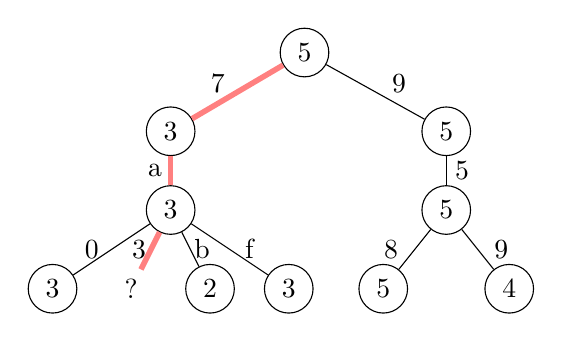
\begin{tikzpicture} [scale=1, auto=left]
    \tikzstyle{selected edge} = [draw,line width=2pt,-,red!50]
    
      \node[circle,draw] (n)       at (4.2,4) {5};
      \node[circle,draw] (n7)     at (2.5,3) {3};
      \node[circle,draw] (n9)     at (6,3)    {5};
      \node[circle,draw] (n7a)   at (2.5,2) {3};
      \node[circle,draw] (n95)   at (6,2)    {5};
      \node[circle,draw] (n7a0) at (1,1)    {3};
      \node(n7a3) at (2,1)    {?};
      \node[circle,draw] (n7ab) at (3,1)    {2};
      \node[circle,draw] (n7af)  at (4,1)    {3};
      \node[circle,draw] (n958) at (5.2,1) {5};
      \node[circle,draw] (n959) at (6.8,1) {4};
    
      \draw[selected edge] (n) -- (n7);
      \draw (n) -- (n9);
      \draw[selected edge] (n7) -- (n7a);
      \draw (n9) -- (n95);
      \draw (n7a) -- (n7a0);
      \draw[selected edge] (n7a) -- (n7a3);
      \draw (n7a) -- (n7ab);
      \draw (n7a) -- (n7af);
      \draw (n95) -- (n958);
      \draw (n95) -- (n959);
      
      \node at (1.5, 1.5) {0};
      \node at (2.1, 1.5) {3};
      \node at (2.9, 1.5) {b};
      \node at (3.5, 1.5) {f};
      
      \node at (5.3, 1.5) {8};
      \node at (6.7, 1.5) {9};
      
      \node at (2.3, 2.5) {a};
      \node at (6.2, 2.5) {5};
      
      \node at (3.1, 3.6) {7};
      \node at (5.4, 3.6) {9};
    \end{tikzpicture}

    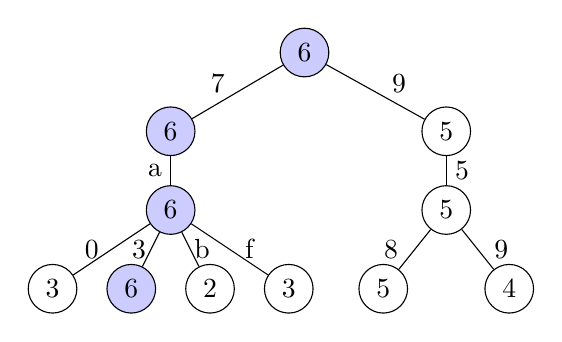
\begin{tikzpicture} [scale=1,auto=left]
      
      \node[circle,draw,fill=blue!20] (n)       at (4.2,4) {6};
      \node[circle,draw,fill=blue!20] (n7)     at (2.5,3) {6};
      \node[circle,draw] (n9)     at (6,3)    {5};
      \node[circle,draw,fill=blue!20] (n7a)   at (2.5,2) {6};
      \node[circle,draw] (n95)   at (6,2)    {5};
      \node[circle,draw] (n7a0) at (1,1)    {3};
      \node[circle,draw,fill=blue!20] (n7a3) at (2,1)    {6};
      \node[circle,draw] (n7ab) at (3,1)    {2};
      \node[circle,draw] (n7af)  at (4,1)    {3};
      \node[circle,draw] (n958) at (5.2,1) {5};
      \node[circle,draw] (n959) at (6.8,1) {4};
    
      \draw (n) -- (n7);
      \draw (n) -- (n9);
      \draw (n7) -- (n7a);
      \draw (n9) -- (n95);
      \draw (n7a) -- (n7a0);
      \draw (n7a) -- (n7a3);
      \draw (n7a) -- (n7ab);
      \draw (n7a) -- (n7af);
      \draw (n95) -- (n958);
      \draw (n95) -- (n959);
      
      \node at (1.5, 1.5) {0};
      \node at (2.1, 1.5) {3};
      \node at (2.9, 1.5) {b};
      \node at (3.5, 1.5) {f};
      
      \node at (5.3, 1.5) {8};
      \node at (6.7, 1.5) {9};
      
      \node at (2.3, 2.5) {a};
      \node at (6.2, 2.5) {5};
      
      \node at (3.1, 3.6) {7};
      \node at (5.4, 3.6) {9};
    \end{tikzpicture}
    

\end{frame} 

\begin{frame}
  \frametitle{Performance Analysis 1/3}

  \begin{itemize}
  \item $d_1$ -- trie depth durung phase 1.

  \item $l$ -- the average leaf size in bytes, counting both key and value.
  For the state tri $l \approx 115$.
  For storage tries $l \approx 42$.
  
  \item $t$ -- total number of leaves in a trie.
  For the state trie it is the number of accounts,
  which is about $53 \cdot 10^6$ as of February 2019.

  \item $m$ -- maximum reply size (approximately), say 32 KiB.
  \end{itemize}

  \bigskip
  
  The overhead of the sync algorithm during phase 1, compared with Parity's warp sync, is in the proof nodes sent alongside the leaf data.
The overhead grows with $d_1$.
On the other hand, small $d_1$ implies a large number of leaves per reply, which can be brittle or inefficient.
During phase~1 an $\texttt{Accounts}$ reply
contains $\frac{t}{16^{d_1}}$ leaves on average,
which gives us
\begin{equation}
    \frac{tl}{16^{d_1}} \leq m
\end{equation}
For the state trie the limit of 32 KiB yields $d_1 = 5$.

\end{frame}

\begin{frame}
  \frametitle{Performance Analysis 2/3}

  \begin{itemize}
    \item $d_2$ -- trie depth durung phase 2.
   
    \item $n$ -- the average node size in bytes.
  Essentially equal to the size of a branch node as most nodes transferred are branch nodes.
  $n \approx 530$.
  
  \item $\delta$ -- the average number of leaf changes per block for a trie.
  For the state trie it is in the ballpark of 300.

  \end{itemize}

  \bigskip
  
  Let $C(d, \delta)$ be the maximum number of trie nodes from the upper $d$ levels of a trie that can change (on average) per block.

  The total reply size per 1 block necessary not to lag behind is no more than
  "Red Queen's Size"
  \begin{equation}
    \texttt{RQS} \overset{\underset{\mathrm{def}}{}}{=}
    C(d_2, \delta) \, n + \delta \, \frac{tl}{16^{d_2}}
\end{equation}

\end{frame}

\begin{frame}
  \frametitle{Performance Analysis 3/3}

  \begin{itemize}
  \item $b$ -- the network bandwidth available to the leecher.
  
  \item $\tau$ -- the block time, currently 15 seconds.

  \end{itemize}

  \bigskip
  
  The value of $d_2$ that minimises $\texttt{RQS}$
  \begin{equation}
      d_2^* = \frac{1}{\ln 16} \ln \left( \frac{tl \ln16}{n} \right)
  \end{equation}
  For the state trie the optimal $d_2^* = 6$ and the entailing $\texttt{RQS}$ is about 0.7 MiB.
  
  The convergence condition for the state trie alone is
  \begin{equation}
      b > \frac{\texttt{RQS}}{\tau}
  \end{equation}
  For the Ethereum main net as of February 2019 this critical minimum bandwidth is about 0.4 Mbit/s.

\end{frame}

\begin{frame}
  \frametitle{Emulation Performance Results}

  STATE TRIE SYNC ONLY
  \bigskip

    \begin{tabular}{ r | c c c }
        Bandwidth & 10M & 50M & 100M \\
        \hline
          1 Mbit/s & 03:39 & 18:44 & 39:04 \\
         10 Mbit/s & 00:20 & 01:39 & 03:17 \\
        100 Mbit/s & 00:02 & 00:10 & 00:20 \\
    \end{tabular}

    \bigskip
  Modelling code and a more formal paper are hosted at
  \href{https://github.com/yperbasis/silkworm/}{https://github.com/yperbasis/silkworm}.


\end{frame}

\end{document}
